\documentclass[12pt]{article}
%Gummi|065|=)
\usepackage{amsmath, amsfonts, amssymb}
\usepackage[margin=0.5in]{geometry}
\usepackage{xcolor}
\usepackage{graphicx}

\newcommand{\off}[1]{}
\DeclareMathSizes{20}{30}{20}{18}

\newcommand{\two }{\sqrt[3]{2}}
\newcommand{\four}{\sqrt[3]{4}}


\usepackage{tikz}

\title{What is Quiver W-Algebra?}
\author{John D Mangual}
\date{}
\begin{document}

\fontfamily{qag}\selectfont \fontsize{12.5}{15}\selectfont

\maketitle

\noindent Here is another situation where I must play ``follow the leader".  Between Pestun, and Kimura, and Nekrasov there's a discussion fo the $qq$-characters and these W-algebras.\footnote{An ``algebra" is just anything with a reasonable addition and multiplication. There are lots and lots of algebras we can use and study. It could be anything.  Yet, I'm confident Vasily knows what he's doing.  Why these?  and more importantly, how can I link these to the stuff that I care about? or to the big discussion?} \\ \\
Why does Pestun and Kimura extend W-algebra in this way?  The only sentence that resonates with me in any way from the intro is ``{\color{red!50!orange}our construction is orthogonal to AGT construction}".  What is AGT?  It is the definition of a conformal field theory, but it is also the literature -- all the research papers that are called ``AGT".  Tody, our discussion will be orthogonal to that. \\ \\
Literally a quiver is a collection of arrows. \\ \\ 
A \textbf{quiver} $\Gamma$ is a set of nodes $\Gamma_0$ and edges $\Gamma_1$.  An \textbf{edge}  from $i$ to $j$ is denoted: $e: i \to j$. \\ \\
A quiver defins a matrix of size $|\Gamma_0 \times \Gamma_0|$ with entries, counting the left and right arrows:
$$ c_{ij} = 2 \delta_{ij} - \# (e: i \to j) - \# (e: j \to i) $$
called the \textbf{quiver Cartan matrix}. 
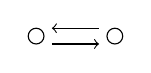
\begin{tikzpicture}
\draw (0,0) circle (0.1);
\draw (1,0) circle (0.1);
\draw[->] (0+0.2,-0.1)--(1-0.2,-0.1);
\draw[<-] (0+0.2,+0.1)--(1-0.2,+0.1);
\end{tikzpicture}
.  Next some quiver jargon:
\begin{itemize}
\item If $c_{ij} = c_{ji}$ ($\# \text{left-pointing arrows}=\# \text{right-pointing arrows}$) the quiver is ``simply laced"
\item If $c_{ij} \neq c_{ji}$ ever, the quiver is ``non-simply laced". 
\end{itemize}
The simply-laced case seems to be old news.  It's not.  We'll discuss both. \\ \\
If the quiver does not have any loops, all diagonal elements $c_{ii} = 2$ (since $\# (i \to i) = 0$).  The Kac-Moody algebras $\mathfrak{g}(\Gamma)$ are ubiquitous in physics.\footnote{``Ubiquitous" is ubiquitous in physics.  In Spanish, the word \textit{ubicar} just means ``located", instead of ``everywhere".} 
\fontfamily{qag}\selectfont \fontsize{10}{15}\selectfont
\begin{quotation}
In mathematics, a \textbf{Kac-Moody algebra} (named for {\color{green!50!white!80!black}Victor Kac} and {\color{blue!50!white}Robert Moody}, who independently discovered them) is a Lie algebra, usually infinite-dimensional, that can be defined by generators and relations through a generalized Cartan matrix. These algebras form a generalization of finite-dimensional semisimple Lie algebras, and many properties related to the structure of a Lie algebra such as its root system, irreducible representations, and connection to flag manifolds have natural analogues in the Kac-Moody setting. \\ \\
A class of Kac-Moody algebras called affine Lie algebras is of particular importance in mathematics and theoretical physics, especially conformal field theory and the theory of exactly solvable models. Kac discovered an elegant proof of certain combinatorial identities, the Macdonald identities, which is based on the representation theory of affine Kac-Moody algebras. \hfill (Wikipedia)
\end{quotation}
\fontfamily{qag}\selectfont \fontsize{12.5}{15}\selectfont
These constructions are rather bland.  We need them to define the \textbf{fractional quiver}.
\newpage

%\noindent I can't stand it !! Make it stop !! Oh God, please make it stop !! \\ \\
\noindent After that unbearable math intro, the physics definition offers us a lot more context.  Just, anything to hold on to.  The examples in Section \textbf{4} look completely tangible and rather fun: \\ \\
\textbf{\#1} $BC_2$ quiver
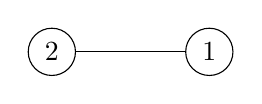
\begin{tikzpicture}
\draw (0,0) circle (0.3);
\node at (0,0) {2};
\draw (2,0) circle (0.3);
\node at (2,0) {1};
\draw (0+0.3,0)--(2-0.3,0);
\end{tikzpicture} has a ``mass-deformed" Cartan matrix:
$$ \left(  \begin{array}{ll} 
1 + \;\; q_1^{-1}q_2^{-2} & - \mu^{-1} \\ 
\hspace{0.1in}-\mu \; q_1^{-1}q_2^{-1}(1+q_2^{-1}) & \;\;\;1 + q_1^{-1}q_2^{-1}
\end{array} \right) \longrightarrow 
\left(  \begin{array}{rr} 
2 & -1 \\ -2 & 2
\end{array} \right)
$$
\textbf{\#2} 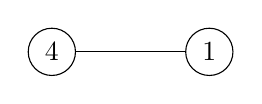
\begin{tikzpicture}
\draw (0,0) circle (0.3);
\node at (0,0) {4};
\draw (2,0) circle (0.3);
\node at (2,0) {1};
\draw (0+0.3,0)--(2-0.3,0);
\end{tikzpicture} the authors call ``affine fractional quiver" with a little more algbra:
$$ \left(  \begin{array}{ll} 
1 + \;\; q_1^{-1}q_2^{-4} & - \mu^{-1} \\ 
\hspace{0.1in}-\mu \; q_1^{-1}q_2^{-1}(1+q_2^{-1}+q_2^{-2} + q_2^{-3}) & \;\;\;1 + q_1^{-1}q_2^{-1}
\end{array} \right) \longrightarrow 
\left(  \begin{array}{rr} 
2 & -1 \\ -4 & 2
\end{array} \right)
$$
\textbf{\#3} 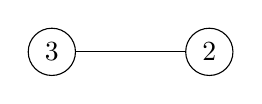
\begin{tikzpicture}
\draw (0,0) circle (0.3);
\node at (0,0) {3};
\draw (2,0) circle (0.3);
\node at (2,0) {2};
\draw (0+0.3,0)--(2-0.3,0);
\end{tikzpicture} the authors call ``hyperbolic fractional quiver"
$$ \left(  \begin{array}{ll} 
1 + \;\; q_1^{-1}q_2^{-3} & - \mu^{-1} \\ 
\hspace{0.1in}-\mu \; q_1^{-1}q_2^{-1}(1+q_2^{-1}+q_2^{-2} ) & \;\;\;1 + q_1^{-1}q_2^{-1}
\end{array} \right) \longrightarrow 
\left(  \begin{array}{rr} 
2 & -2 \\ -3 & 2
\end{array} \right)
$$
This helps us understand what Cartan matrices were all about.  There are $|\Gamma_0| = 2$ notes in each case, and the Cartan matrix is $2 \times 2$.  \\ \\
The $d$-fractional gauge theory on $\mathbb{C}^2$ involves a ring $R = \mathbb{C}[z_1, z_2] $.  At each node, the ring gets replaced by $R_ i= \mathbb{C}[z_1, z_2^{d_i}]$.  Equivariant gauge theory counts $R_i$ ideals.\footnote{Let $R$ be a ring (such as $\mathbb{C}[z_1, z_2]$.  An \textbf{ideal} is a set $\mathfrak{a} \in R$ such that
\begin{itemize}
\item $0 \in \mathfrak{a}$
\item $a,b \in \mathfrak{a}$ implies $a+b \in \mathfrak{a}$
\item $x \in R$ and $a \in \mathfrak{a}$ implies $xa \in \mathfrak{a}$.
\end{itemize} 
This is taken from a Commutative Algebra textbook (e.g. \texttt{http://web.mit.edu/18.705/www/12Nts-2up.pdf})} \\ \\
Once there is a ring you are intersted in, we can consult a Commutative Algebra or Scheme Theory textbook.  Algebraic Geometry really was supposed to be, just Algebra + Geometry
\begin{itemize}
\item we know what Algebra is
\item we know what Geometry is
\end{itemize}
it seems really plausible one might try to solve a geometry problem with algebra (and less frequently the other way around).  And, the great Algebraic Geometers understood that. This is why I really like the textbook of Hodge + Pedoe {\color{red!50!orange}Methods of Algebraic Geometry} and maybe {\color{black!50!white}The Red Book of Varieties and Schemes} by Mumford. \\ \\
I look at a ring like $\mathbb{C}[z_1, z_2]$ and think I know everything there is and could be on that subject. \\ On page 3 of Pestun-Kimura they talk about \textbf{observable sheaves} on the moduli space of instantons associatted to $R_i = \mathbb{C}[z_1, z_2^d]$ \\ \\
This is a great time to review the entire Equivariant Gauge Theory framework presented in Book 1.

\newpage

\noindent \dots 

\vfill

\begin{thebibliography}{}

\item Taro Kimura, Vasily Pestun \textbf{Fractional Quiver W-algebras} \texttt{arXiv:1705.04410}

\item Taro Kimura, Vasily Pestun \textbf{Quiver Elliptic W-algebras} \texttt{arXiv:1608.04651}

\item Taro Kimura, Vasily Pestun \textbf{Quiver W-algebras} \texttt{arXiv:1512.08533}

%\item Nikita Nekrasov. \textbf{BPS/CFT correspondence: non-perturbative Dyson-Schwinger equations and qq-characters.} \texttt{arXiv:1512.05388}





\end{thebibliography}

\end{document}